%%
% Copyright (c) 2017 - 2020, Pascal Wagler;
% Copyright (c) 2014 - 2020, John MacFarlane
%
% All rights reserved.
%
% Redistribution and use in source and binary forms, with or without
% modification, are permitted provided that the following conditions
% are met:
%
% - Redistributions of source code must retain the above copyright
% notice, this list of conditions and the following disclaimer.
%
% - Redistributions in binary form must reproduce the above copyright
% notice, this list of conditions and the following disclaimer in the
% documentation and/or other materials provided with the distribution.
%
% - Neither the name of John MacFarlane nor the names of other
% contributors may be used to endorse or promote products derived
% from this software without specific prior written permission.
%
% THIS SOFTWARE IS PROVIDED BY THE COPYRIGHT HOLDERS AND CONTRIBUTORS
% "AS IS" AND ANY EXPRESS OR IMPLIED WARRANTIES, INCLUDING, BUT NOT
% LIMITED TO, THE IMPLIED WARRANTIES OF MERCHANTABILITY AND FITNESS
% FOR A PARTICULAR PURPOSE ARE DISCLAIMED. IN NO EVENT SHALL THE
% COPYRIGHT OWNER OR CONTRIBUTORS BE LIABLE FOR ANY DIRECT, INDIRECT,
% INCIDENTAL, SPECIAL, EXEMPLARY, OR CONSEQUENTIAL DAMAGES (INCLUDING,
% BUT NOT LIMITED TO, PROCUREMENT OF SUBSTITUTE GOODS OR SERVICES;
% LOSS OF USE, DATA, OR PROFITS; OR BUSINESS INTERRUPTION) HOWEVER
% CAUSED AND ON ANY THEORY OF LIABILITY, WHETHER IN CONTRACT, STRICT
% LIABILITY, OR TORT (INCLUDING NEGLIGENCE OR OTHERWISE) ARISING IN
% ANY WAY OUT OF THE USE OF THIS SOFTWARE, EVEN IF ADVISED OF THE
% POSSIBILITY OF SUCH DAMAGE.
%%

%%
% This is the Eisvogel pandoc LaTeX template.
%
% For usage information and examples visit the official GitHub page:
% https://github.com/Wandmalfarbe/pandoc-latex-template
%%

\DeclareUnicodeCharacter{2212}{-}

% Options for packages loaded elsewhere
\PassOptionsToPackage{unicode}{hyperref}
\PassOptionsToPackage{hyphens}{url}
\PassOptionsToPackage{dvipsnames,svgnames*,x11names*,table}{xcolor}
%
\documentclass[
  12pt,
  a4paper,
,tablecaptionabove
]{scrartcl}
\usepackage{lmodern}
\usepackage{setspace}
\setstretch{1.2}
\usepackage{amssymb,amsmath}
\usepackage{ifxetex,ifluatex}
\ifnum 0\ifxetex 1\fi\ifluatex 1\fi=0 % if pdftex
  \usepackage[T1]{fontenc}
  \usepackage[utf8]{inputenc}
  \usepackage{textcomp} % provide euro and other symbols
\else % if luatex or xetex
  \usepackage{unicode-math}
  \defaultfontfeatures{Scale=MatchLowercase}
  \defaultfontfeatures[\rmfamily]{Ligatures=TeX,Scale=1}
\fi
% Use upquote if available, for straight quotes in verbatim environments
\IfFileExists{upquote.sty}{\usepackage{upquote}}{}
\IfFileExists{microtype.sty}{% use microtype if available
  \usepackage[]{microtype}
  \UseMicrotypeSet[protrusion]{basicmath} % disable protrusion for tt fonts
}{}
\makeatletter
\@ifundefined{KOMAClassName}{% if non-KOMA class
  \IfFileExists{parskip.sty}{%
    \usepackage{parskip}
  }{% else
    \setlength{\parindent}{0pt}
    \setlength{\parskip}{6pt plus 2pt minus 1pt}}
}{% if KOMA class
  \KOMAoptions{parskip=half}}
\makeatother
\usepackage{xcolor}
\definecolor{default-linkcolor}{HTML}{A50000}
\definecolor{default-filecolor}{HTML}{A50000}
\definecolor{default-citecolor}{HTML}{4077C0}
\definecolor{default-urlcolor}{HTML}{4077C0}
\IfFileExists{xurl.sty}{\usepackage{xurl}}{} % add URL line breaks if available
\IfFileExists{bookmark.sty}{\usepackage{bookmark}}{\usepackage{hyperref}}
\hypersetup{
  pdftitle={Katabuchi et al., Decomposing leaf mass into metabolic and structural components explains divergent patterns of trait variation within and among plant species},
  colorlinks=true,
  linkcolor=blue,
  filecolor=default-filecolor,
  citecolor=default-citecolor,
  urlcolor=default-urlcolor,
  breaklinks=true,
  pdfcreator={LaTeX via pandoc with the Eisvogel template}}
\urlstyle{same} % disable monospaced font for URLs
\usepackage[margin=1in]{geometry}
\usepackage{color}
\usepackage{fancyvrb}
\newcommand{\VerbBar}{|}
\newcommand{\VERB}{\Verb[commandchars=\\\{\}]}
\DefineVerbatimEnvironment{Highlighting}{Verbatim}{commandchars=\\\{\}}
% Add ',fontsize=\small' for more characters per line
\usepackage{framed}
\definecolor{shadecolor}{RGB}{241,243,245}
\newenvironment{Shaded}{\begin{snugshade}}{\end{snugshade}}
\newcommand{\AlertTok}[1]{\textcolor[rgb]{0.68,0.00,0.00}{#1}}
\newcommand{\AnnotationTok}[1]{\textcolor[rgb]{0.37,0.37,0.37}{#1}}
\newcommand{\AttributeTok}[1]{\textcolor[rgb]{0.40,0.45,0.13}{#1}}
\newcommand{\BaseNTok}[1]{\textcolor[rgb]{0.68,0.00,0.00}{#1}}
\newcommand{\BuiltInTok}[1]{\textcolor[rgb]{0.00,0.23,0.31}{#1}}
\newcommand{\CharTok}[1]{\textcolor[rgb]{0.13,0.47,0.30}{#1}}
\newcommand{\CommentTok}[1]{\textcolor[rgb]{0.37,0.37,0.37}{#1}}
\newcommand{\CommentVarTok}[1]{\textcolor[rgb]{0.37,0.37,0.37}{\textit{#1}}}
\newcommand{\ConstantTok}[1]{\textcolor[rgb]{0.56,0.35,0.01}{#1}}
\newcommand{\ControlFlowTok}[1]{\textcolor[rgb]{0.00,0.23,0.31}{#1}}
\newcommand{\DataTypeTok}[1]{\textcolor[rgb]{0.68,0.00,0.00}{#1}}
\newcommand{\DecValTok}[1]{\textcolor[rgb]{0.68,0.00,0.00}{#1}}
\newcommand{\DocumentationTok}[1]{\textcolor[rgb]{0.37,0.37,0.37}{\textit{#1}}}
\newcommand{\ErrorTok}[1]{\textcolor[rgb]{0.68,0.00,0.00}{#1}}
\newcommand{\ExtensionTok}[1]{\textcolor[rgb]{0.00,0.23,0.31}{#1}}
\newcommand{\FloatTok}[1]{\textcolor[rgb]{0.68,0.00,0.00}{#1}}
\newcommand{\FunctionTok}[1]{\textcolor[rgb]{0.28,0.35,0.67}{#1}}
\newcommand{\ImportTok}[1]{\textcolor[rgb]{0.00,0.46,0.62}{#1}}
\newcommand{\InformationTok}[1]{\textcolor[rgb]{0.37,0.37,0.37}{#1}}
\newcommand{\KeywordTok}[1]{\textcolor[rgb]{0.00,0.23,0.31}{#1}}
\newcommand{\NormalTok}[1]{\textcolor[rgb]{0.00,0.23,0.31}{#1}}
\newcommand{\OperatorTok}[1]{\textcolor[rgb]{0.37,0.37,0.37}{#1}}
\newcommand{\OtherTok}[1]{\textcolor[rgb]{0.00,0.23,0.31}{#1}}
\newcommand{\PreprocessorTok}[1]{\textcolor[rgb]{0.68,0.00,0.00}{#1}}
\newcommand{\RegionMarkerTok}[1]{\textcolor[rgb]{0.00,0.23,0.31}{#1}}
\newcommand{\SpecialCharTok}[1]{\textcolor[rgb]{0.37,0.37,0.37}{#1}}
\newcommand{\SpecialStringTok}[1]{\textcolor[rgb]{0.13,0.47,0.30}{#1}}
\newcommand{\StringTok}[1]{\textcolor[rgb]{0.13,0.47,0.30}{#1}}
\newcommand{\VariableTok}[1]{\textcolor[rgb]{0.07,0.07,0.07}{#1}}
\newcommand{\VerbatimStringTok}[1]{\textcolor[rgb]{0.13,0.47,0.30}{#1}}
\newcommand{\WarningTok}[1]{\textcolor[rgb]{0.37,0.37,0.37}{\textit{#1}}}

% Workaround/bugfix from jannick0.
% See https://github.com/jgm/pandoc/issues/4302#issuecomment-360669013)
% or https://github.com/Wandmalfarbe/pandoc-latex-template/issues/2
%
% Redefine the verbatim environment 'Highlighting' to break long lines (with
% the help of fvextra). Redefinition is necessary because it is unlikely that
% pandoc includes fvextra in the default template.
\usepackage{fvextra}
\DefineVerbatimEnvironment{Highlighting}{Verbatim}{breaklines,fontsize=\small,commandchars=\\\{\}}

\usepackage{longtable,booktabs}
% Correct order of tables after \paragraph or \subparagraph
\usepackage{etoolbox}
\makeatletter
\patchcmd\longtable{\par}{\if@noskipsec\mbox{}\fi\par}{}{}
\makeatother
% Allow footnotes in longtable head/foot
\IfFileExists{footnotehyper.sty}{\usepackage{footnotehyper}}{\usepackage{footnote}}
\makesavenoteenv{longtable}
% add backlinks to footnote references, cf. https://tex.stackexchange.com/questions/302266/make-footnote-clickable-both-ways
\usepackage{footnotebackref}
\usepackage{graphicx}
\makeatletter
\def\maxwidth{\ifdim\Gin@nat@width>\linewidth\linewidth\else\Gin@nat@width\fi}
\def\maxheight{\ifdim\Gin@nat@height>\textheight\textheight\else\Gin@nat@height\fi}
\makeatother
% Scale images if necessary, so that they will not overflow the page
% margins by default, and it is still possible to overwrite the defaults
% using explicit options in \includegraphics[width, height, ...]{}
\setkeys{Gin}{width=\maxwidth,height=\maxheight,keepaspectratio}
\setlength{\emergencystretch}{3em}  % prevent overfull lines
\providecommand{\tightlist}{%
  \setlength{\itemsep}{0pt}\setlength{\parskip}{0pt}}
\setcounter{secnumdepth}{-\maxdimen} % remove section numbering
% Make \paragraph and \subparagraph free-standing
\ifx\paragraph\undefined\else
  \let\oldparagraph\paragraph
  \renewcommand{\paragraph}[1]{\oldparagraph{#1}\mbox{}}
\fi
\ifx\subparagraph\undefined\else
  \let\oldsubparagraph\subparagraph
  \renewcommand{\subparagraph}[1]{\oldsubparagraph{#1}\mbox{}}
\fi

% Make use of float-package and set default placement for figures to H.
% The option H means 'PUT IT HERE' (as  opposed to the standard h option which means 'You may put it here if you like').
\usepackage{float}
\floatplacement{figure}{H}

\usepackage{booktabs}
\usepackage{longtable}
\usepackage{array}
\usepackage{multirow}
\usepackage{wrapfig}
\usepackage{float}
\usepackage{colortbl}
\usepackage{pdflscape}
\usepackage{tabu}
\usepackage{threeparttable}
\usepackage{threeparttablex}
\usepackage[normalem]{ulem}
\usepackage{makecell}
\usepackage{xcolor}
\makeatletter
\makeatother
\makeatletter
\makeatother
\makeatletter
\@ifpackageloaded{caption}{}{\usepackage{caption}}
\AtBeginDocument{%
\ifdefined\contentsname
  \renewcommand*\contentsname{Table of contents}
\else
  \newcommand\contentsname{Table of contents}
\fi
\ifdefined\listfigurename
  \renewcommand*\listfigurename{List of Figures}
\else
  \newcommand\listfigurename{List of Figures}
\fi
\ifdefined\listtablename
  \renewcommand*\listtablename{List of Tables}
\else
  \newcommand\listtablename{List of Tables}
\fi
\ifdefined\figurename
  \renewcommand*\figurename{Figure}
\else
  \newcommand\figurename{Figure}
\fi
\ifdefined\tablename
  \renewcommand*\tablename{Table}
\else
  \newcommand\tablename{Table}
\fi
}
\@ifpackageloaded{float}{}{\usepackage{float}}
\floatstyle{ruled}
\@ifundefined{c@chapter}{\newfloat{codelisting}{h}{lop}}{\newfloat{codelisting}{h}{lop}[chapter]}
\floatname{codelisting}{Listing}
\newcommand*\listoflistings{\listof{codelisting}{List of Listings}}
\makeatother
\makeatletter
\@ifpackageloaded{caption}{}{\usepackage{caption}}
\@ifpackageloaded{subcaption}{}{\usepackage{subcaption}}
\makeatother
\makeatletter
\@ifpackageloaded{tcolorbox}{}{\usepackage[many]{tcolorbox}}
\makeatother
\makeatletter
\@ifundefined{shadecolor}{\definecolor{shadecolor}{rgb}{.97, .97, .97}}
\makeatother
\makeatletter
\makeatother

\newlength{\cslhangindent}
\setlength{\cslhangindent}{1.5em}
\newlength{\csllabelwidth}
\setlength{\csllabelwidth}{3em}
\newenvironment{CSLReferences}[2] % #1 hanging-ident, #2 entry spacing
 {% don't indent paragraphs
  \setlength{\parindent}{0pt}
  % turn on hanging indent if param 1 is 1
  \ifodd #1 \everypar{\setlength{\hangindent}{\cslhangindent}}\ignorespaces\fi
  % set entry spacing
  \ifnum #2 > 0
  \setlength{\parskip}{#2\baselineskip}
  \fi
 }%
 {}
\usepackage{calc}
\newcommand{\CSLBlock}[1]{#1\hfill\break}
\newcommand{\CSLLeftMargin}[1]{\parbox[t]{\csllabelwidth}{#1}}
\newcommand{\CSLRightInline}[1]{\parbox[t]{\linewidth - \csllabelwidth}{#1}\break}
\newcommand{\CSLIndent}[1]{\hspace{\cslhangindent}#1}

\title{Katabuchi et al., Decomposing leaf mass into metabolic and
structural components explains divergent patterns of trait variation
within and among plant species}
\date{}


%%
%% added
%%

%
% language specification
%
% If no language is specified, use English as the default main document language.
%

\ifnum 0\ifxetex 1\fi\ifluatex 1\fi=0 % if pdftex
  \usepackage[shorthands=off,main=english]{babel}
\else
    % Workaround for bug in Polyglossia that breaks `\familydefault` when `\setmainlanguage` is used.
  % See https://github.com/Wandmalfarbe/pandoc-latex-template/issues/8
  % See https://github.com/reutenauer/polyglossia/issues/186
  % See https://github.com/reutenauer/polyglossia/issues/127
  \renewcommand*\familydefault{\sfdefault}
    % load polyglossia as late as possible as it *could* call bidi if RTL lang (e.g. Hebrew or Arabic)
  \usepackage{polyglossia}
  \setmainlanguage[]{english}
\fi



%
% for the background color of the title page
%

%
% break urls
%
\PassOptionsToPackage{hyphens}{url}

%
% When using babel or polyglossia with biblatex, loading csquotes is recommended
% to ensure that quoted texts are typeset according to the rules of your main language.
%
\usepackage{csquotes}

%
% captions
%
%\definecolor{caption-color}{HTML}{777777}
\definecolor{caption-color}{HTML}{37474F}
%\usepackage[font={stretch=1.2}, textfont={color=caption-color}, position=top, skip=4mm, labelfont=bf, singlelinecheck=false, justification=raggedright]{caption}
\usepackage[font={stretch=1}, textfont={color=caption-color}, position=top, skip=2mm, labelfont=bf, singlelinecheck=false, justification=raggedright]{caption}
\setcapindent{0em}

%
% blockquote
%
\definecolor{blockquote-border}{RGB}{221,221,221}
\definecolor{blockquote-text}{RGB}{119,119,119}
\usepackage{mdframed}
\newmdenv[rightline=false,bottomline=false,topline=false,linewidth=3pt,linecolor=blockquote-border,skipabove=\parskip]{customblockquote}
\renewenvironment{quote}{\begin{customblockquote}\list{}{\rightmargin=0em\leftmargin=0em}%
\item\relax\color{blockquote-text}\ignorespaces}{\unskip\unskip\endlist\end{customblockquote}}

%
% Source Sans Pro as the de­fault font fam­ily
% Source Code Pro for monospace text
%
% 'default' option sets the default
% font family to Source Sans Pro, not \sfdefault.
%
\ifnum 0\ifxetex 1\fi\ifluatex 1\fi=0 % if pdftex
    \usepackage[default]{sourcesanspro}
  \usepackage{sourcecodepro}
  %\usepackage{}
  \else % if not pdftex
    \usepackage[default]{sourcesanspro}
  \usepackage{sourcecodepro}
  %\usepackage{}

  % XeLaTeX specific adjustments for straight quotes: https://tex.stackexchange.com/a/354887
  % This issue is already fixed (see https://github.com/silkeh/latex-sourcecodepro/pull/5) but the
  % fix is still unreleased.
  % TODO: Remove this workaround when the new version of sourcecodepro is released on CTAN.
  \ifxetex
    \makeatletter
    \defaultfontfeatures[\ttfamily]
      { Numbers   = \sourcecodepro@figurestyle,
        Scale     = \SourceCodePro@scale,
        Extension = .otf }
    \setmonofont
      [ UprightFont    = *-\sourcecodepro@regstyle,
        ItalicFont     = *-\sourcecodepro@regstyle It,
        BoldFont       = *-\sourcecodepro@boldstyle,
        BoldItalicFont = *-\sourcecodepro@boldstyle It ]
      {SourceCodePro}
    \makeatother
  \fi
  \fi

%
% heading color
%
\definecolor{heading-color}{RGB}{40,40,40}
\addtokomafont{section}{\color{heading-color}}
% When using the classes report, scrreprt, book,
% scrbook or memoir, uncomment the following line.
%\addtokomafont{chapter}{\color{heading-color}}

%
% variables for title and author
%
\usepackage{titling}
\title{Katabuchi et al., Decomposing leaf mass into metabolic and
structural components explains divergent patterns of trait variation
within and among plant species}
\author{}

%
% tables
%

\definecolor{table-row-color}{HTML}{F5F5F5}
\definecolor{table-rule-color}{HTML}{999999}

%\arrayrulecolor{black!40}
\arrayrulecolor{table-rule-color}     % color of \toprule, \midrule, \bottomrule
\setlength\heavyrulewidth{0.3ex}      % thickness of \toprule, \bottomrule
\renewcommand{\arraystretch}{1.3}     % spacing (padding)


%
% remove paragraph indention
%
\setlength{\parindent}{0pt}
\setlength{\parskip}{6pt plus 2pt minus 1pt}
\setlength{\emergencystretch}{3em}  % prevent overfull lines

%
%
% Listings
%
%


%
% header and footer
%
\usepackage{fancyhdr}

\fancypagestyle{eisvogel-header-footer}{
  \fancyhead{}
  \fancyfoot{}
  \lhead[]{Katabuchi et al., Decomposing leaf mass into metabolic and
structural components explains divergent patterns of trait variation
within and among plant species}
  \chead[]{}
  \rhead[Katabuchi et al., Decomposing leaf mass into metabolic and
structural components explains divergent patterns of trait variation
within and among plant species]{}
  %\lfoot[\thepage]{}
  \cfoot[]{}
  \cfoot[]{\thepage}
  \renewcommand{\headrulewidth}{0.0pt}
 % \renewcommand{\footrulewidth}{0.0pt}
 % \renewcommand{\headrulewidth}{0.4pt}
 % \renewcommand{\footrulewidth}{0.4pt}
}
\pagestyle{eisvogel-header-footer}

%%
%% end added
%%

\begin{document}

%%
%% begin titlepage
%%

%%
%% end titlepage
%%



\ifdefined\Shaded\renewenvironment{Shaded}{\begin{tcolorbox}[boxrule=0pt, breakable, interior hidden, borderline west={3pt}{0pt}{shadecolor}, frame hidden, sharp corners, enhanced]}{\end{tcolorbox}}\fi

\newpage

\hypertarget{appendix-s1-prior-information}{%
\section{Appendix S1: Prior
information}\label{appendix-s1-prior-information}}

The logarithms of \emph{A}\textsubscript{area},
\emph{R}\textsubscript{area}, and LL for leaf sample \emph{i} were
assumed to have a multivariate normal distribution as following:

\begin{align}
\left(
\begin{array}{ccc}
\mathrm{ln}[A_{\mathrm{area} \, i}]\\
\mathrm{ln}[R_{\mathrm{area} \, i}] \\
\mathrm{ln}[\mathrm{LL}_i]
\end{array}
\right)
\sim \mathrm{MVN}
\left(
\begin{array}{rrr}
\mathrm{E}[A_{\mathrm{area} \, i}]\\
\mathrm{E}[R_{\mathrm{area} \, i}] &, \boldsymbol{\Sigma}\\
\mathrm{E}[\mathrm{LL}_i]
\end{array}
\right) \tag{S1}
\end{align}

where E{[}\(\cdot\){]} indicates expected value; \(\boldsymbol{\Sigma}\)
indicates a covariance matrix. Expected values are based on Eqs. 1-6 in
the main text.

We used non-informative or weakly informative prior distributions
(\protect\hyperlink{ref-Lemoine2019}{Lemoine 2019}). The covariance
mkatrix in Eq. S1 was decomposed as
\({\mathbf \Sigma} = {\mathrm diag}({\mathbf \sigma}){\mathbf \Omega}{\mathrm diag}({\mathbf \sigma}) = {\mathrm diag}({\mathbf \sigma}){\mathbf L}{\mathbf L}\prime {\mathrm diag}({\mathbf \sigma})\)
using a Cholesky decomposition, where \({\mathbf \sigma}\) is a vector
of \(\sigma_{1}\), \(\sigma_{2}\), and \(\sigma_{3}\);
\({\mathbf \Omega}\) is a correlation matrix of \(\rho_{12}\),
\(\rho_{13}\), and \(\rho_{23}\); and \textbf{L} is a lower triangular
matrix. Instead of assigning prior distributions on directly, priors
were assigned on and \textbf{L} to avoid a strong dependence between and
(\protect\hyperlink{ref-Lewandowski2009}{Lewandowski et al. 2009},
\protect\hyperlink{ref-Alvarez2014}{Alvarez et al. 2014}). A prior for
\textbf{L} was specified as a so-called LKJ distribution with shape
parameter 2 (\protect\hyperlink{ref-Lewandowski2009}{Lewandowski et al.
2009}), which is weakly informative for the correlation matrix. A prior
for \({\mathrm diag}({\mathbf \sigma})\) was specified as a Half-Cauchy
distribution with location 0 and scale 5, which is weakly informative
and allows for occasional large coefficients while still performing a
reasonable amount of shrinkage for coefficients near zero
(\protect\hyperlink{ref-Gelman2008}{Gelman et al. 2008}). A prior for
\(\mathbf{\sigma}\) was specified as a Half-Cauchy distribution with
location 0 and scale 5, which is weakly informative and allows for
occasional large coefficients while still performing a reasonable amount
of shrinkage for coefficients near zero
(\protect\hyperlink{ref-Gelman2008}{Gelman et al. 2008}). Priors for
\(\alpha_{0,p,s}\), \(\beta_{0,p,s}\), and \(\gamma_{0,p,s}\) in Eqs.
4-6 were weakly informative and specified as normal distributions with
mean 0 and standard deviation 5. Priors for \emph{f\textsubscript{i}} in
Eqs. 4-6 were non-informative and specified as uniform distributions
with range (0, 1).

\newpage

\hypertarget{appendix-s2-randomization-including-table-as1-and-figure-as1}{%
\section{Appendix S2: Randomization (including Table AS1 and Figure
AS1)}\label{appendix-s2-randomization-including-table-as1-and-figure-as1}}

We generated 10 randomized datasets for each of the GLOPNET and the
Panama datasets by shuffling each trait value across leaf samples, and
fit the best models (Appendix S1) to the randomized data.

\hypertarget{table-as1}{%
\subsection{Table AS1}\label{table-as1}}

\begin{itemize}
\tightlist
\item
  No\_large\_Rhat: The number of parameters (including transformed
  parameters) that shows Rhat (Gelman-Rubin statistic) greater than
  1.05.
\item
  No\_divergence: The number of iterations that shows divergent
  transitions.
\end{itemize}

\begin{longtable}[]{@{}lrrr@{}}
\toprule()
Data & Simulation\_ID & No\_large\_Rhat & No\_divergence \\
\midrule()
\endhead
GLOPNET & 1 & 261 & 516 \\
GLOPNET & 2 & 0 & 17 \\
GLOPNET & 3 & 0 & 5 \\
GLOPNET & 4 & 0 & 32 \\
GLOPNET & 5 & 510 & 208 \\
GLOPNET & 6 & 458 & 34 \\
GLOPNET & 7 & 0 & 14 \\
GLOPNET & 8 & 7 & 4 \\
GLOPNET & 9 & 52 & 1 \\
GLOPNET & 10 & 1086 & 25 \\
Panama & 1 & 842 & 429 \\
Panama & 2 & 657 & 14 \\
Panama & 3 & 408 & 76 \\
Panama & 4 & 846 & 44 \\
Panama & 5 & 966 & 1213 \\
Panama & 6 & 829 & 90 \\
Panama & 7 & 262 & 73 \\
Panama & 8 & 641 & 128 \\
Panama & 9 & 900 & 77 \\
Panama & 10 & 623 & 301 \\
\bottomrule()
\end{longtable}

Model results obtained from the randomized datasets did not convergent
based on the Gelman-Rubin statistic or showed divergent transitions.

\newpage

\hypertarget{figure-as1}{%
\subsection{Figure AS1}\label{figure-as1}}

Although divergent transitions suggesting that the posterior
distribution is not reliable, we checked the regression coefficients for
GLOPNET (\(\alpha_{0, p, s}\), \(\beta_{0, s}\), and
\(\gamma_{0, p, s}\) in Eqs. 4-6 in the main text). There are 10
independent simulations (randomizations) in total. The simulation ID 2,
3, 4 and 7 were convergent based on the Gelman-Rubin statistic, but
those randomized datasets did not show any patterns. Thus, the tests
with randomized data indicate that our model is not inherently prone to
overfitting or to producing patterns from noise.

\includegraphics{../figs/coef_rand.png}

\newpage

\hypertarget{figure-s1}{%
\section{Figure S1}\label{figure-s1}}

Pearson correlation coefficients for posterior medians of LMAp vs LMAs
in the (a) GLOPNET and (b) Panama datasets. The non-significant or weak
\emph{r} values indicate that a single axis could not accurately
represent the two-dimensional space. Symbols as in Main Text Figs. 1-2.

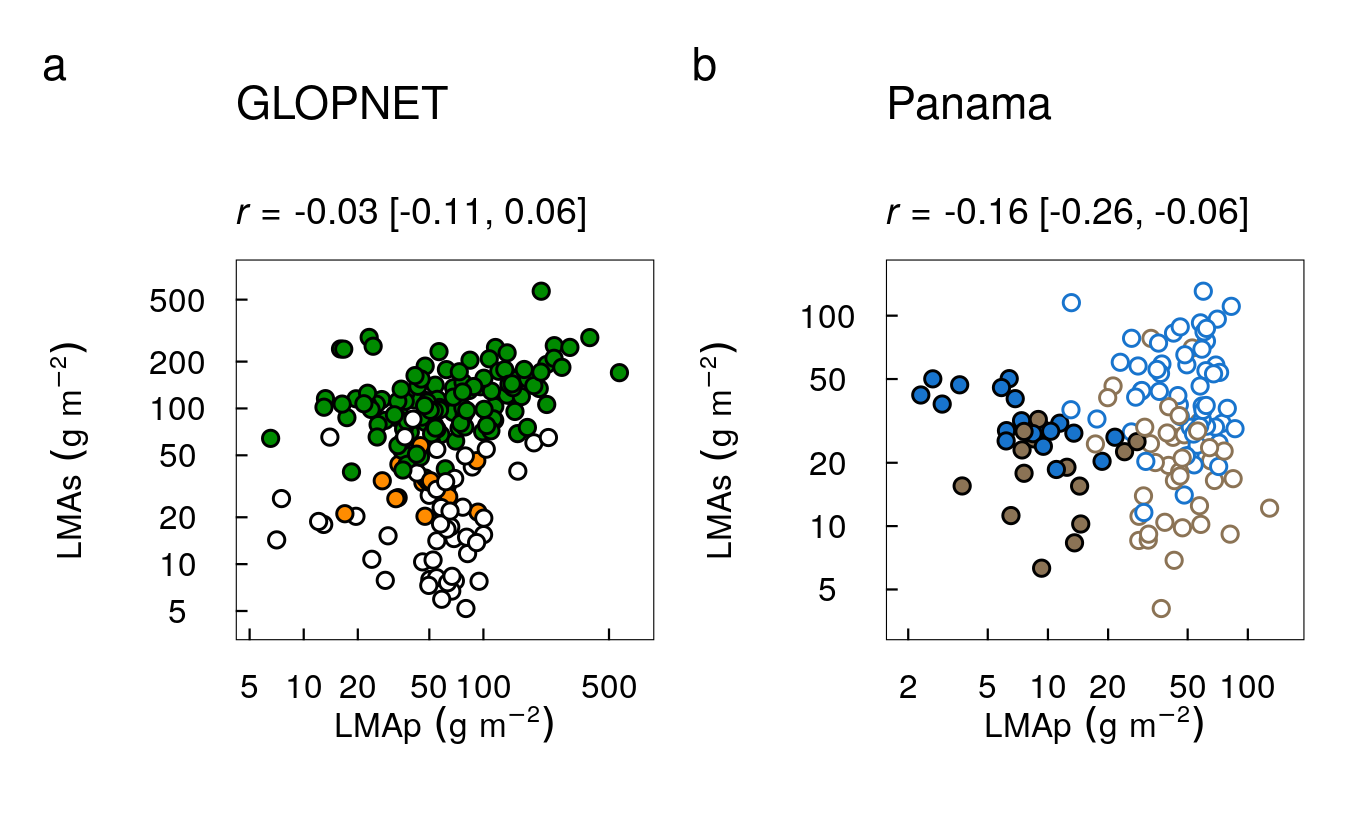
\includegraphics{../figs/ps_point.png}

\newpage

\hypertarget{figure-s2}{%
\section{Figure S2}\label{figure-s2}}

Boxplots comparing leaf mass per area (LMA), photosynthetic leaf mass
per area (LMAp; posterior means), and structural leaf mass per area
(LMAs; posterior means) across sites (wet and dry) and canopy strata
(sun and shade) in Panama. The results shown here include all leaves in
the Panama dataset, whereas Fig. 5 in the main text only includes Panama
species for which both sun and shade leaves were available. Boxplot
symbols as in Fig. 5. Groups sharing the same letters are not
significantly different (P \textgreater{} 0.05; t-tests).

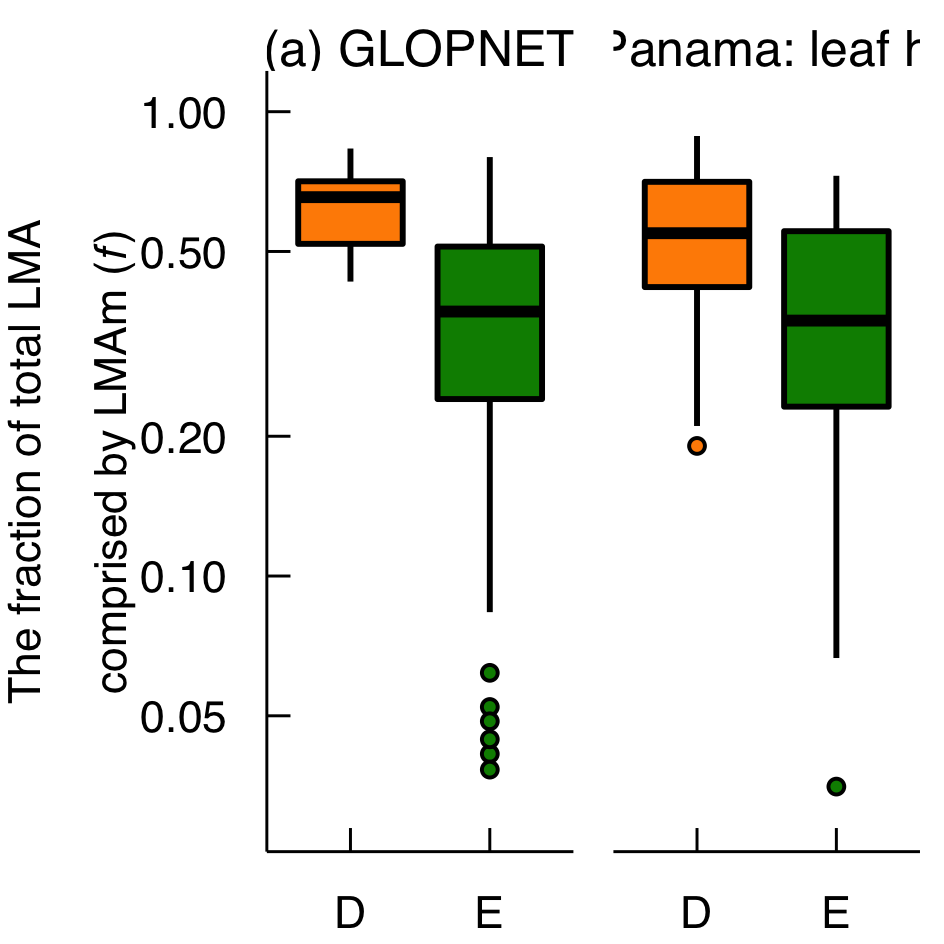
\includegraphics{../figs/box_frac.png}

\newpage

\hypertarget{figure-s2-1}{%
\section{Figure S2}\label{figure-s2-1}}

Boxplots comparing leaf mass per area (LMA), photosynthetic leaf mass
per area (LMAp; posterior means), and structural leaf mass per area
(LMAs; posterior means) across sites (wet and dry) and canopy strata
(sun and shade) in Panama. The results shown here include all leaves in
the Panama dataset, whereas Fig. 5 in the main text only includes Panama
species for which both sun and shade leaves were available. Boxplot
symbols as in Fig. 5. Groups sharing the same letters are not
significantly different (P \textgreater{} 0.05; t-tests).

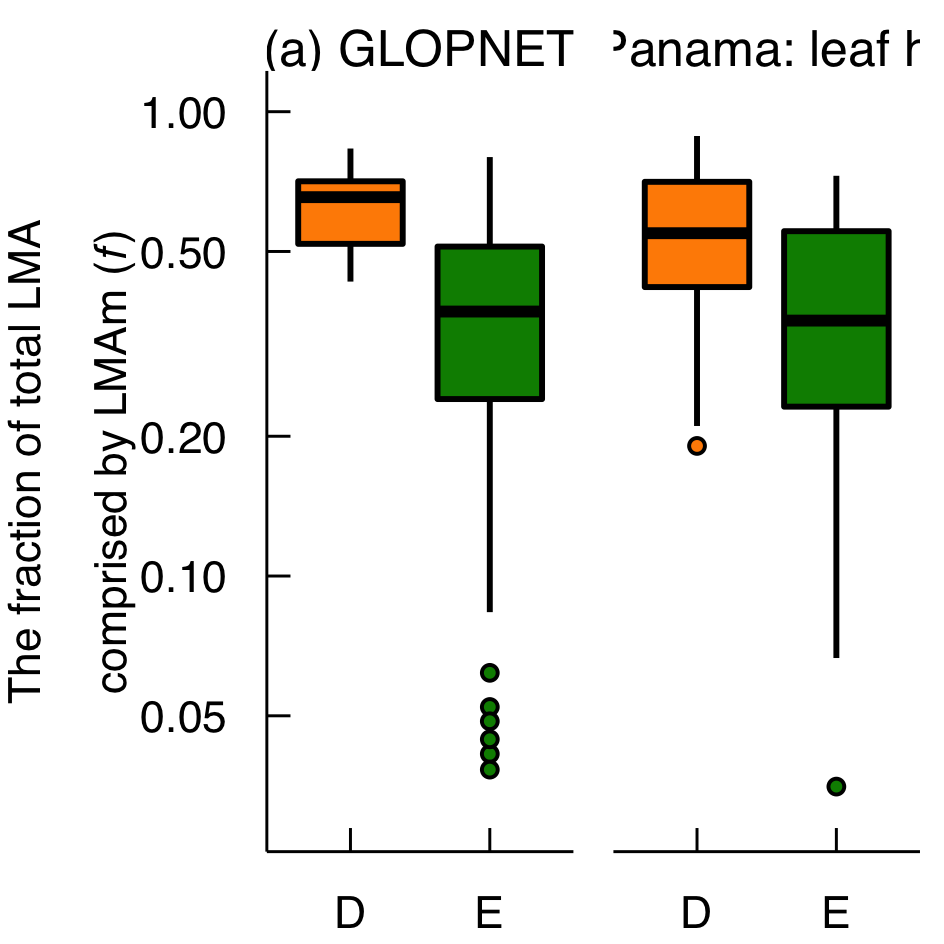
\includegraphics{../figs/box_frac.png}

\newpage

\hypertarget{figure-s3}{%
\section{Figure S3}\label{figure-s3}}

Mass-prop

\newpage

\hypertarget{figure-s4}{%
\section{Figure S4}\label{figure-s4}}

Measured traits related to photosynthesis and metabolism (nitrogen and
phosphorus per-unit leaf area; \emph{N}\textsubscript{area} and
\emph{P}\textsubscript{area}) are positively correlated with LMA and
with estimates (posterior means) of the photosynthetic and structural
LMA components (LMAp and LMAs, respectively) in the GLOPNET dataset.
LMAp yields stronger correlations and more consistent relationships
compared to LMA and LMAs; e.g., evergreen and deciduous leaves align
along a single relationship in panel b, but not in panels a or c.

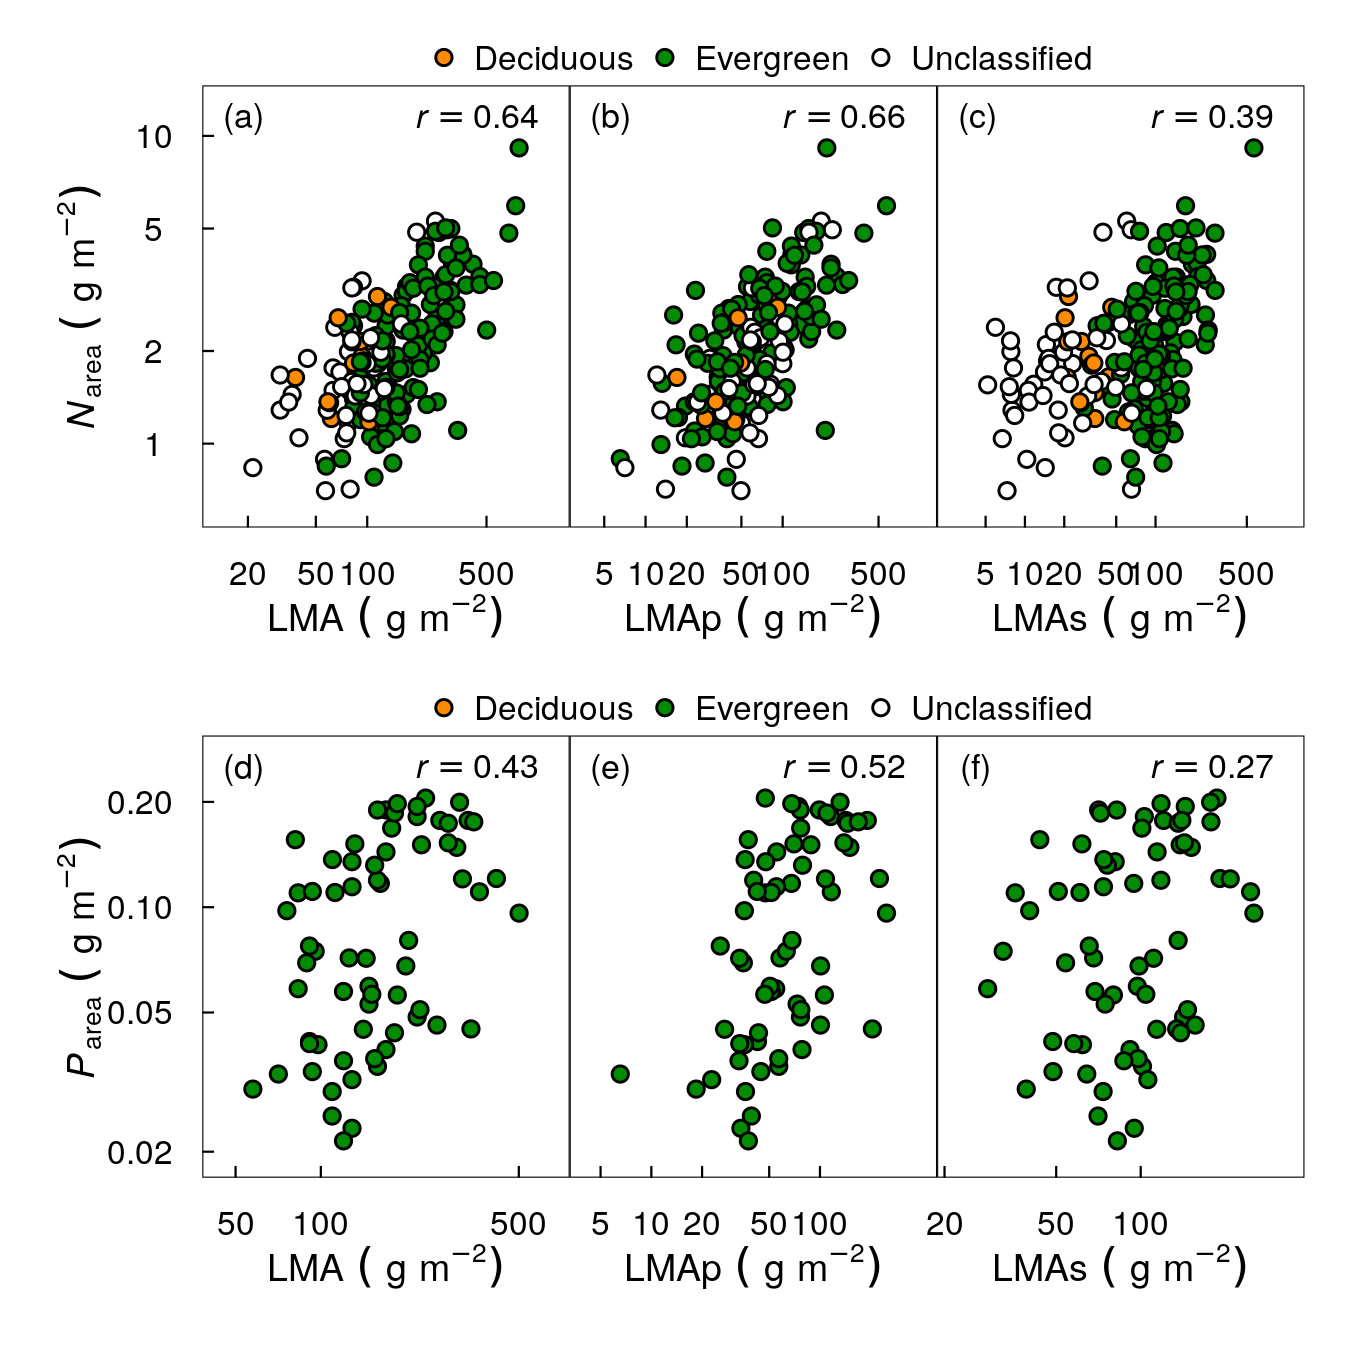
\includegraphics{../figs/gl_point_np2.png}

\hypertarget{appendix-s3-stan-code}{%
\section{Appendix S3: Stan code}\label{appendix-s3-stan-code}}

\hypertarget{stan-code-for-the-glopnet-dataset}{%
\subsection{Stan code for the GLOPNET
dataset}\label{stan-code-for-the-glopnet-dataset}}

The best model for the GLOPNET dataset is (2) LMAp and LMAs, and (b)
\(\alpha_p > \alpha_s\) and \(\beta_p = 0\).

\begin{Shaded}
\begin{Highlighting}[]
\CommentTok{//}\AlertTok{NOTE}\CommentTok{: THIS STAN CODE IS GENERATED VIA "update.py"}
\KeywordTok{data}\NormalTok{\{}
  \DataTypeTok{int}\NormalTok{\textless{}}\KeywordTok{lower}\NormalTok{=}\DecValTok{0}\NormalTok{\textgreater{} N;}
  \DataTypeTok{vector}\NormalTok{\textless{}}\KeywordTok{lower}\NormalTok{=}\DecValTok{0}\NormalTok{\textgreater{}[N] LMA;}
  \DataTypeTok{vector}\NormalTok{\textless{}}\KeywordTok{lower}\NormalTok{=}\DecValTok{0}\NormalTok{\textgreater{}[N] A;}
  \DataTypeTok{vector}\NormalTok{\textless{}}\KeywordTok{lower}\NormalTok{=}\DecValTok{0}\NormalTok{\textgreater{}[N] R;}
  \DataTypeTok{vector}\NormalTok{\textless{}}\KeywordTok{lower}\NormalTok{=}\DecValTok{0}\NormalTok{\textgreater{}[N] LL;}
\NormalTok{\}}
\KeywordTok{transformed data}\NormalTok{\{}
  \DataTypeTok{vector}\NormalTok{[N] log\_A;}
  \DataTypeTok{vector}\NormalTok{[N] log\_LL;}
  \DataTypeTok{vector}\NormalTok{[N] log\_R;}
  \DataTypeTok{matrix}\NormalTok{[N,}\DecValTok{3}\NormalTok{] obs;}
  \DataTypeTok{vector}\NormalTok{[N] intercept;}
  \ControlFlowTok{for}\NormalTok{ (n }\ControlFlowTok{in} \DecValTok{1}\NormalTok{:N)}
\NormalTok{    intercept[n] = }\DecValTok{1}\NormalTok{;}
\NormalTok{  log\_A = log(A);}
\NormalTok{  log\_LL = log(LL);}
\NormalTok{  log\_R = log(R);}
  \CommentTok{// use net photosynthesis (A) instead of gross (A + R)}
\NormalTok{  obs = append\_col(append\_col(log\_A, log\_LL), log\_R);}
\NormalTok{\}}

\KeywordTok{parameters}\NormalTok{\{}
  \DataTypeTok{real}\NormalTok{ a0;}
  \DataTypeTok{real}\NormalTok{ ap;}
  \DataTypeTok{real}\NormalTok{\textless{}}\KeywordTok{upper}\NormalTok{=ap\textgreater{} as;}
  \DataTypeTok{real}\NormalTok{ b0;}
  \DataTypeTok{real}\NormalTok{ bs;}
  \DataTypeTok{real}\NormalTok{ g0;}
  \DataTypeTok{real}\NormalTok{ gp;}
  \DataTypeTok{real}\NormalTok{ gs;}
  \DataTypeTok{vector}\NormalTok{\textless{}}\KeywordTok{lower}\NormalTok{=}\DecValTok{0}\NormalTok{, }\KeywordTok{upper}\NormalTok{=}\DecValTok{1}\NormalTok{\textgreater{}[N] p;}
  \DataTypeTok{vector}\NormalTok{\textless{}}\KeywordTok{lower}\NormalTok{=}\DecValTok{0}\NormalTok{\textgreater{}[}\DecValTok{3}\NormalTok{] L\_sigma;}
  \DataTypeTok{cholesky\_factor\_corr}\NormalTok{[}\DecValTok{3}\NormalTok{] L\_Omega;}
\NormalTok{\}}
\KeywordTok{transformed parameters}\NormalTok{\{}
  \DataTypeTok{matrix}\NormalTok{[N,}\DecValTok{3}\NormalTok{] Mu;}
  \DataTypeTok{matrix}\NormalTok{[}\DecValTok{3}\NormalTok{,}\DecValTok{3}\NormalTok{] Z;}
  \DataTypeTok{matrix}\NormalTok{[N,}\DecValTok{3}\NormalTok{] X;}
  \DataTypeTok{matrix}\NormalTok{[N,}\DecValTok{3}\NormalTok{] L\_Sigma;}
\NormalTok{  Z[}\DecValTok{1}\NormalTok{,}\DecValTok{1}\NormalTok{] = a0;}
\NormalTok{  Z[}\DecValTok{1}\NormalTok{,}\DecValTok{2}\NormalTok{] = b0;}
\NormalTok{  Z[}\DecValTok{1}\NormalTok{,}\DecValTok{3}\NormalTok{] = g0;}
\NormalTok{  Z[}\DecValTok{2}\NormalTok{,}\DecValTok{1}\NormalTok{] = ap;}
\NormalTok{  Z[}\DecValTok{2}\NormalTok{,}\DecValTok{2}\NormalTok{] = }\DecValTok{0}\NormalTok{;}
\NormalTok{  Z[}\DecValTok{2}\NormalTok{,}\DecValTok{3}\NormalTok{] = gp;}
\NormalTok{  Z[}\DecValTok{3}\NormalTok{,}\DecValTok{1}\NormalTok{] = as;}
\NormalTok{  Z[}\DecValTok{3}\NormalTok{,}\DecValTok{2}\NormalTok{] = bs;}
\NormalTok{  Z[}\DecValTok{3}\NormalTok{,}\DecValTok{3}\NormalTok{] = gs;}

\NormalTok{  L\_Sigma = rep\_matrix(to\_row\_vector(}\FloatTok{0.5}\NormalTok{ * L\_sigma .* L\_sigma), N);}
  \CommentTok{//log\_LMAp = log(LMA) + log(p);}
  \CommentTok{//log\_LMAs = log(LMA) + log(1 {-} p);}
  \CommentTok{//X = append\_col(append\_col(append\_col(intercept, log\_LMAp), log\_LMAs), leaf);}
\NormalTok{  X = append\_col(append\_col(intercept, log(LMA) + log(p)), log(LMA) + log(}\DecValTok{1}\NormalTok{ {-} p));}
\NormalTok{  Mu = X * Z {-} L\_Sigma;}
\NormalTok{\}}
\KeywordTok{model}\NormalTok{\{}
  \CommentTok{// priors}
\NormalTok{  a0 \textasciitilde{} normal(}\DecValTok{0}\NormalTok{, }\DecValTok{5}\NormalTok{);}
\NormalTok{  b0 \textasciitilde{} normal(}\DecValTok{0}\NormalTok{, }\DecValTok{5}\NormalTok{);}
\NormalTok{  g0 \textasciitilde{} normal(}\DecValTok{0}\NormalTok{, }\DecValTok{5}\NormalTok{);}
\NormalTok{  ap \textasciitilde{} normal(}\DecValTok{0}\NormalTok{, }\DecValTok{5}\NormalTok{);}
\NormalTok{  bs \textasciitilde{} normal(}\DecValTok{0}\NormalTok{, }\DecValTok{5}\NormalTok{);}
\NormalTok{  gp \textasciitilde{} normal(}\DecValTok{0}\NormalTok{, }\DecValTok{5}\NormalTok{);}
\NormalTok{  gs \textasciitilde{} normal(}\DecValTok{0}\NormalTok{, }\DecValTok{5}\NormalTok{);}
\NormalTok{  as \textasciitilde{} normal(}\DecValTok{0}\NormalTok{, }\DecValTok{5}\NormalTok{);}
\NormalTok{  p \textasciitilde{} beta(}\DecValTok{1}\NormalTok{, }\DecValTok{1}\NormalTok{);}
\NormalTok{  L\_Omega \textasciitilde{} lkj\_corr\_cholesky(}\DecValTok{2}\NormalTok{); }\CommentTok{//uniform of L\_Omega * L\_Omega\textquotesingle{}}
\NormalTok{  L\_sigma \textasciitilde{} cauchy(}\DecValTok{0}\NormalTok{, }\DecValTok{5}\NormalTok{);}

  \CommentTok{// model}
  \ControlFlowTok{for}\NormalTok{ (i }\ControlFlowTok{in} \DecValTok{1}\NormalTok{:N)}
     \KeywordTok{target +=}\NormalTok{ multi\_normal\_cholesky\_lpdf(obs[i,] | Mu[i,], diag\_pre\_multiply(L\_sigma, L\_Omega));}
\NormalTok{\}}
\KeywordTok{generated quantities}\NormalTok{ \{}
  \DataTypeTok{vector}\NormalTok{[N] log\_lik;}
  \DataTypeTok{real}\NormalTok{\textless{}}\KeywordTok{lower}\NormalTok{={-}}\DecValTok{1}\NormalTok{, }\KeywordTok{upper}\NormalTok{=}\DecValTok{1}\NormalTok{\textgreater{} rho12;}
  \DataTypeTok{real}\NormalTok{\textless{}}\KeywordTok{lower}\NormalTok{={-}}\DecValTok{1}\NormalTok{, }\KeywordTok{upper}\NormalTok{=}\DecValTok{1}\NormalTok{\textgreater{} rho23;}
  \DataTypeTok{real}\NormalTok{\textless{}}\KeywordTok{lower}\NormalTok{={-}}\DecValTok{1}\NormalTok{, }\KeywordTok{upper}\NormalTok{=}\DecValTok{1}\NormalTok{\textgreater{} rho13;}
  \DataTypeTok{cov\_matrix}\NormalTok{[}\DecValTok{3}\NormalTok{] Sigma;}
\NormalTok{  Sigma = diag\_pre\_multiply(L\_sigma, L\_Omega)}
\NormalTok{     * diag\_post\_multiply(L\_Omega\textquotesingle{}, L\_sigma);}
\NormalTok{  rho12 = Sigma[}\DecValTok{1}\NormalTok{, }\DecValTok{2}\NormalTok{] * inv(L\_sigma[}\DecValTok{1}\NormalTok{] * L\_sigma[}\DecValTok{2}\NormalTok{]);}
\NormalTok{  rho23 = Sigma[}\DecValTok{2}\NormalTok{, }\DecValTok{3}\NormalTok{] * inv(L\_sigma[}\DecValTok{2}\NormalTok{] * L\_sigma[}\DecValTok{3}\NormalTok{]);}
\NormalTok{  rho13 = Sigma[}\DecValTok{1}\NormalTok{, }\DecValTok{3}\NormalTok{] * inv(L\_sigma[}\DecValTok{1}\NormalTok{] * L\_sigma[}\DecValTok{3}\NormalTok{]);}
  \ControlFlowTok{for}\NormalTok{ (i }\ControlFlowTok{in} \DecValTok{1}\NormalTok{:N)}
\NormalTok{   log\_lik[i] = multi\_normal\_cholesky\_lpdf(obs[i,] | Mu[i,], diag\_pre\_multiply(L\_sigma, L\_Omega));}
\NormalTok{ \}}
\end{Highlighting}
\end{Shaded}

\hypertarget{stan-code-for-the-panama-dataset}{%
\subsection{Stan code for the Panama
dataset}\label{stan-code-for-the-panama-dataset}}

The best model for the Panama dataset is (4) LMAp, LMAs and light, and
(a) \(\alpha_s = 0\) and \(\beta_p = 0\),

\begin{Shaded}
\begin{Highlighting}[]
\CommentTok{//}\AlertTok{NOTE}\CommentTok{: THIS STAN CODE IS GENERATED VIA "update.py"}
\KeywordTok{data}\NormalTok{\{}
  \DataTypeTok{int}\NormalTok{\textless{}}\KeywordTok{lower}\NormalTok{=}\DecValTok{0}\NormalTok{\textgreater{} N;}
  \DataTypeTok{vector}\NormalTok{\textless{}}\KeywordTok{lower}\NormalTok{=}\DecValTok{0}\NormalTok{\textgreater{}[N] LMA;}
  \DataTypeTok{vector}\NormalTok{\textless{}}\KeywordTok{lower}\NormalTok{=}\DecValTok{0}\NormalTok{\textgreater{}[N] A;}
  \DataTypeTok{vector}\NormalTok{\textless{}}\KeywordTok{lower}\NormalTok{=}\DecValTok{0}\NormalTok{\textgreater{}[N] R;}
  \DataTypeTok{vector}\NormalTok{\textless{}}\KeywordTok{lower}\NormalTok{=}\DecValTok{0}\NormalTok{\textgreater{}[N] LL;}
  \DataTypeTok{vector}\NormalTok{\textless{}}\KeywordTok{lower}\NormalTok{=}\DecValTok{0}\NormalTok{\textgreater{}[N] leaf;}
\NormalTok{\}}
\KeywordTok{transformed data}\NormalTok{\{}
  \DataTypeTok{vector}\NormalTok{[N] log\_A;}
  \DataTypeTok{vector}\NormalTok{[N] log\_LL;}
  \DataTypeTok{vector}\NormalTok{[N] log\_R;}
  \DataTypeTok{matrix}\NormalTok{[N,}\DecValTok{3}\NormalTok{] obs;}
  \DataTypeTok{vector}\NormalTok{[N] intercept;}
  \ControlFlowTok{for}\NormalTok{ (n }\ControlFlowTok{in} \DecValTok{1}\NormalTok{:N)}
\NormalTok{    intercept[n] = }\DecValTok{1}\NormalTok{;}
\NormalTok{  log\_A = log(A);}
\NormalTok{  log\_LL = log(LL);}
\NormalTok{  log\_R = log(R);}
  \CommentTok{// use net photosynthesis (A) instead of gross (A + R)}
\NormalTok{  obs = append\_col(append\_col(log\_A, log\_LL), log\_R);}
\NormalTok{\}}

\KeywordTok{parameters}\NormalTok{\{}
  \DataTypeTok{real}\NormalTok{ a0;}
  \DataTypeTok{real}\NormalTok{ ap;}
  \DataTypeTok{real}\NormalTok{ b0;}
  \DataTypeTok{real}\NormalTok{ bs;}
  \DataTypeTok{real}\NormalTok{ g0;}
  \DataTypeTok{real}\NormalTok{ gp;}
  \DataTypeTok{real}\NormalTok{ gs;}
  \DataTypeTok{real}\NormalTok{ theta;}
  \DataTypeTok{vector}\NormalTok{\textless{}}\KeywordTok{lower}\NormalTok{=}\DecValTok{0}\NormalTok{, }\KeywordTok{upper}\NormalTok{=}\DecValTok{1}\NormalTok{\textgreater{}[N] p;}
  \DataTypeTok{vector}\NormalTok{\textless{}}\KeywordTok{lower}\NormalTok{=}\DecValTok{0}\NormalTok{\textgreater{}[}\DecValTok{3}\NormalTok{] L\_sigma;}
  \DataTypeTok{cholesky\_factor\_corr}\NormalTok{[}\DecValTok{3}\NormalTok{] L\_Omega;}
\NormalTok{\}}
\KeywordTok{transformed parameters}\NormalTok{\{}
  \DataTypeTok{matrix}\NormalTok{[N,}\DecValTok{3}\NormalTok{] Mu;}
  \DataTypeTok{matrix}\NormalTok{[}\DecValTok{4}\NormalTok{,}\DecValTok{3}\NormalTok{] Z;}
  \DataTypeTok{matrix}\NormalTok{[N,}\DecValTok{4}\NormalTok{] X;}
  \DataTypeTok{matrix}\NormalTok{[N,}\DecValTok{3}\NormalTok{] L\_Sigma;}
\NormalTok{  Z[}\DecValTok{1}\NormalTok{,}\DecValTok{1}\NormalTok{] = a0;}
\NormalTok{  Z[}\DecValTok{1}\NormalTok{,}\DecValTok{2}\NormalTok{] = b0;}
\NormalTok{  Z[}\DecValTok{1}\NormalTok{,}\DecValTok{3}\NormalTok{] = g0;}
\NormalTok{  Z[}\DecValTok{2}\NormalTok{,}\DecValTok{1}\NormalTok{] = ap;}
\NormalTok{  Z[}\DecValTok{2}\NormalTok{,}\DecValTok{2}\NormalTok{] = }\DecValTok{0}\NormalTok{;}
\NormalTok{  Z[}\DecValTok{2}\NormalTok{,}\DecValTok{3}\NormalTok{] = gp;}
\NormalTok{  Z[}\DecValTok{3}\NormalTok{,}\DecValTok{1}\NormalTok{] = }\DecValTok{0}\NormalTok{;}
\NormalTok{  Z[}\DecValTok{3}\NormalTok{,}\DecValTok{2}\NormalTok{] = bs;}
\NormalTok{  Z[}\DecValTok{3}\NormalTok{,}\DecValTok{3}\NormalTok{] = gs;}
\NormalTok{  Z[}\DecValTok{4}\NormalTok{,}\DecValTok{1}\NormalTok{] = }\DecValTok{0}\NormalTok{;}
\NormalTok{  Z[}\DecValTok{4}\NormalTok{,}\DecValTok{2}\NormalTok{] = theta;}
\NormalTok{  Z[}\DecValTok{4}\NormalTok{,}\DecValTok{3}\NormalTok{] = }\DecValTok{0}\NormalTok{;}

\NormalTok{  L\_Sigma = rep\_matrix(to\_row\_vector(}\FloatTok{0.5}\NormalTok{ * L\_sigma .* L\_sigma), N);}
  \CommentTok{//log\_LMAp = log(LMA) + log(p);}
  \CommentTok{//log\_LMAs = log(LMA) + log(1 {-} p);}
  \CommentTok{//X = append\_col(append\_col(append\_col(intercept, log\_LMAp), log\_LMAs), leaf);}
\NormalTok{  X = append\_col(append\_col(append\_col(intercept,}
\NormalTok{    log(LMA) + log(p)),}
\NormalTok{    log(LMA) + log(}\DecValTok{1}\NormalTok{ {-} p)),}
\NormalTok{     leaf);}
\NormalTok{  Mu = X * Z {-} L\_Sigma;}
\NormalTok{\}}
\KeywordTok{model}\NormalTok{\{}
  \CommentTok{// priors}
\NormalTok{  a0 \textasciitilde{} normal(}\DecValTok{0}\NormalTok{, }\DecValTok{5}\NormalTok{);}
\NormalTok{  b0 \textasciitilde{} normal(}\DecValTok{0}\NormalTok{, }\DecValTok{5}\NormalTok{);}
\NormalTok{  g0 \textasciitilde{} normal(}\DecValTok{0}\NormalTok{, }\DecValTok{5}\NormalTok{);}
\NormalTok{  ap \textasciitilde{} normal(}\DecValTok{0}\NormalTok{, }\DecValTok{5}\NormalTok{);}
\NormalTok{  bs \textasciitilde{} normal(}\DecValTok{0}\NormalTok{, }\DecValTok{5}\NormalTok{);}
\NormalTok{  gp \textasciitilde{} normal(}\DecValTok{0}\NormalTok{, }\DecValTok{5}\NormalTok{);}
\NormalTok{  gs \textasciitilde{} normal(}\DecValTok{0}\NormalTok{, }\DecValTok{5}\NormalTok{);}
\NormalTok{  theta \textasciitilde{} normal(}\DecValTok{0}\NormalTok{, }\DecValTok{5}\NormalTok{);}
\NormalTok{  p \textasciitilde{} beta(}\DecValTok{1}\NormalTok{, }\DecValTok{1}\NormalTok{);}
\NormalTok{  L\_Omega \textasciitilde{} lkj\_corr\_cholesky(}\DecValTok{2}\NormalTok{); }\CommentTok{//uniform of L\_Omega * L\_Omega\textquotesingle{}}
\NormalTok{  L\_sigma \textasciitilde{} cauchy(}\DecValTok{0}\NormalTok{, }\DecValTok{5}\NormalTok{);}

  \CommentTok{// model}
  \ControlFlowTok{for}\NormalTok{ (i }\ControlFlowTok{in} \DecValTok{1}\NormalTok{:N)}
     \KeywordTok{target +=}\NormalTok{ multi\_normal\_cholesky\_lpdf(obs[i,] | Mu[i,], diag\_pre\_multiply(L\_sigma, L\_Omega));}
\NormalTok{\}}
\KeywordTok{generated quantities}\NormalTok{ \{}
  \DataTypeTok{vector}\NormalTok{[N] log\_lik;}
  \DataTypeTok{real}\NormalTok{\textless{}}\KeywordTok{lower}\NormalTok{={-}}\DecValTok{1}\NormalTok{, }\KeywordTok{upper}\NormalTok{=}\DecValTok{1}\NormalTok{\textgreater{} rho12;}
  \DataTypeTok{real}\NormalTok{\textless{}}\KeywordTok{lower}\NormalTok{={-}}\DecValTok{1}\NormalTok{, }\KeywordTok{upper}\NormalTok{=}\DecValTok{1}\NormalTok{\textgreater{} rho23;}
  \DataTypeTok{real}\NormalTok{\textless{}}\KeywordTok{lower}\NormalTok{={-}}\DecValTok{1}\NormalTok{, }\KeywordTok{upper}\NormalTok{=}\DecValTok{1}\NormalTok{\textgreater{} rho13;}
  \DataTypeTok{cov\_matrix}\NormalTok{[}\DecValTok{3}\NormalTok{] Sigma;}
\NormalTok{  Sigma = diag\_pre\_multiply(L\_sigma, L\_Omega)}
\NormalTok{     * diag\_post\_multiply(L\_Omega\textquotesingle{}, L\_sigma);}
\NormalTok{  rho12 = Sigma[}\DecValTok{1}\NormalTok{, }\DecValTok{2}\NormalTok{] * inv(L\_sigma[}\DecValTok{1}\NormalTok{] * L\_sigma[}\DecValTok{2}\NormalTok{]);}
\NormalTok{  rho23 = Sigma[}\DecValTok{2}\NormalTok{, }\DecValTok{3}\NormalTok{] * inv(L\_sigma[}\DecValTok{2}\NormalTok{] * L\_sigma[}\DecValTok{3}\NormalTok{]);}
\NormalTok{  rho13 = Sigma[}\DecValTok{1}\NormalTok{, }\DecValTok{3}\NormalTok{] * inv(L\_sigma[}\DecValTok{1}\NormalTok{] * L\_sigma[}\DecValTok{3}\NormalTok{]);}
  \ControlFlowTok{for}\NormalTok{ (i }\ControlFlowTok{in} \DecValTok{1}\NormalTok{:N)}
\NormalTok{   log\_lik[i] = multi\_normal\_cholesky\_lpdf(obs[i,] | Mu[i,], diag\_pre\_multiply(L\_sigma, L\_Omega));}
\NormalTok{ \}}
\end{Highlighting}
\end{Shaded}

\hypertarget{references}{%
\section*{References}\label{references}}
\addcontentsline{toc}{section}{References}

\hypertarget{refs}{}
\begin{CSLReferences}{1}{0}
\leavevmode\vadjust pre{\hypertarget{ref-Alvarez2014}{}}%
Alvarez, I., J. Niemi, and M. Simpson. 2014.
\href{https://doi.org/10.1214/aos/1176348885}{Bayesian inference for a
covariance matrix}. arXiv preprint arXiv:1408.4050v2:1--12.

\leavevmode\vadjust pre{\hypertarget{ref-Gelman2008}{}}%
Gelman, A., A. Jakulin, M. G. Pittau, and Y. S. Su. 2008.
\href{https://doi.org/10.1214/08-AOAS191}{A weakly informative default
prior distribution for logistic and other regression models}. Annals of
Applied Statistics 2:1360--1383.

\leavevmode\vadjust pre{\hypertarget{ref-Lemoine2019}{}}%
Lemoine, N. P. 2019. \href{https://doi.org/10.1111/oik.05985}{Moving
beyond noninformative priors: Why and how to choose weakly informative
priors in {Bayesian} analyses}. Oikos 128:912--928.

\leavevmode\vadjust pre{\hypertarget{ref-Lewandowski2009}{}}%
Lewandowski, D., D. Kurowicka, and H. Joe. 2009.
\href{https://doi.org/10.1016/j.jmva.2009.04.008}{Generating random
correlation matrices based on vines and extended onion method}. Journal
of Multivariate Analysis 100:1989--2001.

\end{CSLReferences}

\end{document}
